% FIG ch04-04b schematic labels (Chinese)
\usetikzlibrary{positioning}
\begin{tikzpicture}
\node[anchor=south west,inner sep=0] (img) at (0,0) {%
  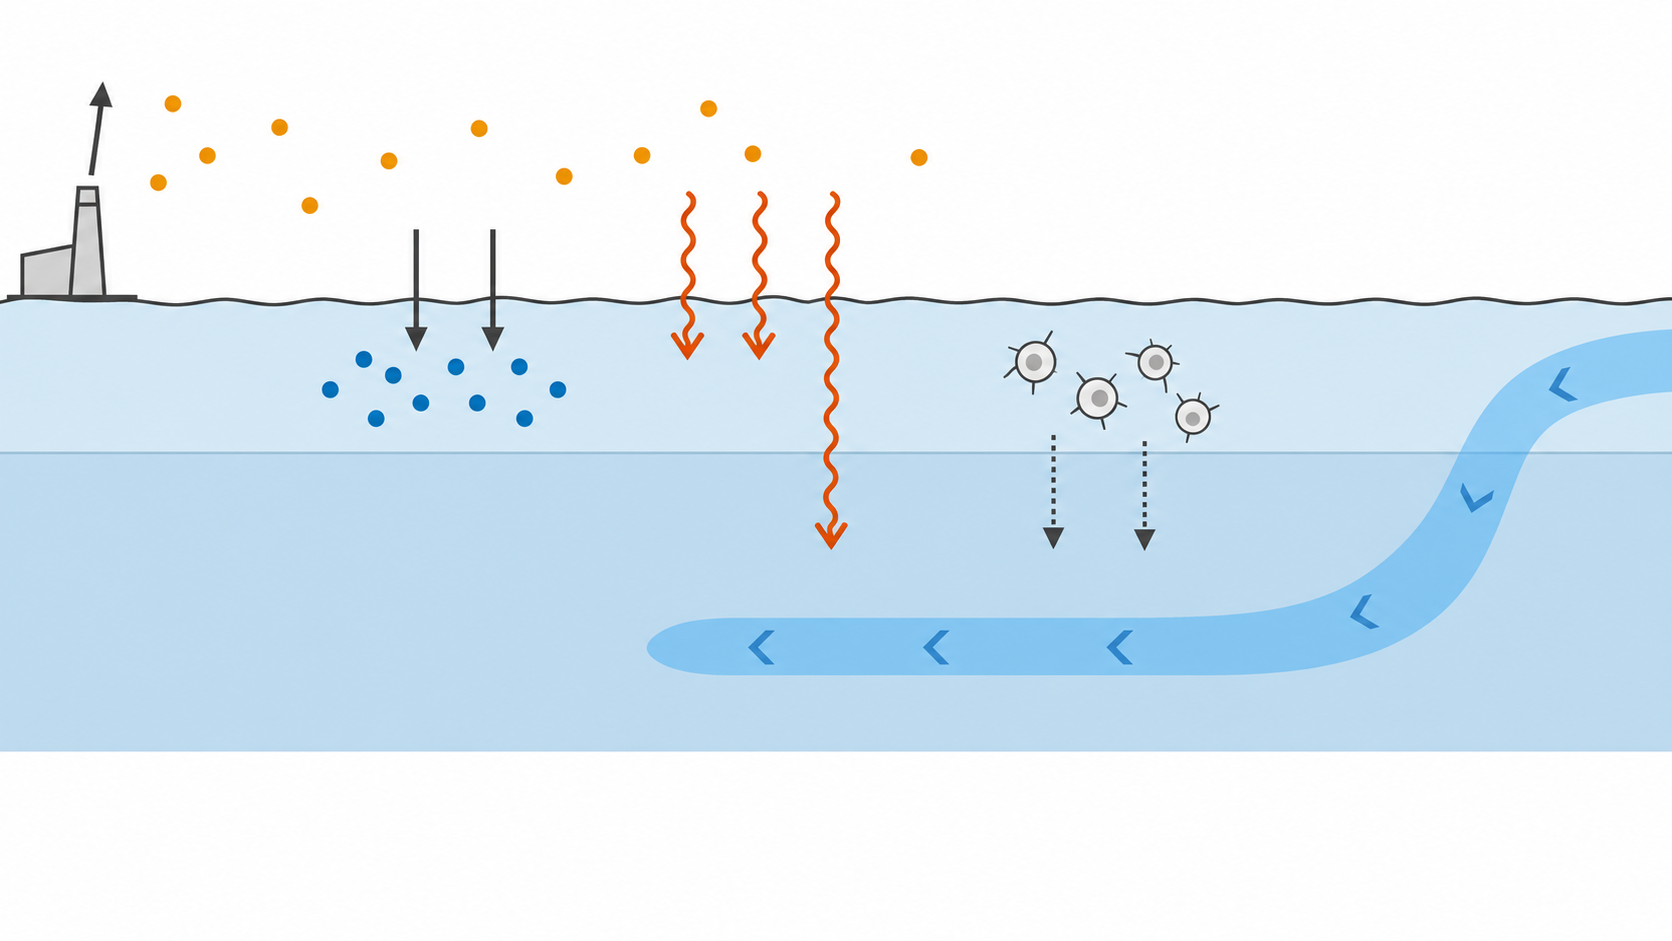
\includegraphics[width=\linewidth]{figures/ch04/ch04-04b-schematic-base.png}};
\begin{scope}[x={(img.south east)},y={(img.north west)},font=\sffamily\small]
  \node at (0.92,0.90) {大气};
  \node at (0.92,0.66) {表层混合层};
  \node at (0.92,0.35) {海洋内部};
  \node[align=left] at (0.06,0.93) {人为排放};
  \node at (0.30,0.88) {CO\textsubscript{2}};
  \node at (0.33,0.70) {海气交换};
  \node at (0.30,0.60) {溶解无机碳};
  \node at (0.55,0.70) {热量吸收};
  \node[align=center] at (0.80,0.45) {水体下沉\\与输运};
  \node at (0.48,0.62) {浮游植物};
  \node[align=center] at (0.48,0.42) {下沉颗粒\\（生物泵）};
  \node[align=center,font=\scriptsize] at (0.50,0.04) {%
    图例：碳通量 / 热通量 / 水体输运 / 下沉颗粒};
\end{scope}
\end{tikzpicture}
